\documentclass{beamer}
\mode<presentation>
\usetheme{CambridgeUS}
\usepackage[russian]{babel}
\usepackage[utf8]{inputenc}
\usepackage[T2A]{fontenc}
\usepackage{sansmathaccent}

\usepackage{verbatim}
\usepackage{alltt}

%\pdfmapfile{+sansmathaccent.map}
\title[Artifical Intelligence]{Ассоциативные правила}
\author{Наумов Д.А., доц. каф. КТ}
\date[22.11.2020] {Экспертные системы и искусственный интеллект, 2020}

\begin{document}

%ТИТУЛЬНЫЙ СЛАЙД
\begin{frame}
  \titlepage
\end{frame}
  
%СОДЕРЖАНИЕ ЛЕКЦИИ
\begin{frame}
  \frametitle{Содержание лекции}
  \tableofcontents  
\end{frame}

\section{Задачи поиска ассоциативных правил}

\begin{frame}{Что такое поиск ассоциативных правил?}
	\begin{block}{Поиск ассоциативных правил}
		поиск часто в страчающихся шаблонов, ассоциаций, корреляций или структур среди множества элементов в транзакционной базе данных.
	\end{block}
	Понять покупательские привычки клиента, находя ассоциации и корреляции между различными товарами, которые клиенты размещают в их <<корзину для покупок>>. 

	Практическое применение:
	\begin{itemize}
		\item анализ покупок;
		\item кросс-маркетинг;
		\item каталогизация;
		\item web-анализ;
		\item обнаружение мошеннических схем.
	\end{itemize} 
\end{frame}

\begin{frame}{Что такое поиск ассоциативных правил?}
	\begin{block}{Ассоциативное правило}
		\begin{figure}[h]
			\centering
			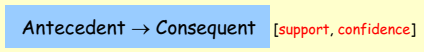
\includegraphics[scale=0.75]{images/lec08-pic01.png}
		\end{figure}
	\end{block}
	\begin{itemize}
		\item Antecedent -- антецедент, причина;
		\item Consequent -- косеквент, следствие;
		\item Support -- поддержка (мера интересности правила);
		\item Confedence -- значимость (мера интересности правила).
	\end{itemize} 
	Примеры:
		\[buys(x, "computer") \rightarrow buys(x, "financial management software")\]
		\[[0.5\%, 60\%]\]
		\[age(x, "30..39") and income(x, "42..48K") \rightarrow buys(x, "car")\]
		\[[1\%,75\%]\]
\end{frame}

\begin{frame}{Как можно использовать ассоциативные правила?}
	\begin{itemize}
		\item пусть правило имеет вид:
		\begin{figure}[h]
  			\centering
  			
\includegraphics[scale=0.9]{images/lec08-pic03.png}
		\end{figure}
		\item \textbf{Potato chips} (следствие) -- продажи чего мы собираемся (можем) увеличивать;
		\item \textbf{Bagels} (антецедент) -- какие продукты будут влиять на продажу, если объявить скидки;
		\item \textbf{Bagels} -> \textbf{Potato chips} -- какие продукты следует размещать рядом, чтобы увеличить продажи Potato Chips.
	\end{itemize}

	Практическое применение:
	\begin{itemize}
		\item оптимизировать размещение товара на полках;
		\item формировать персональные рекомендации;
		\item планирование промо-акции;
		\item более эффективно управлять ценами и ассортиментом.
	\end{itemize}
\end{frame}

\begin{frame}{Ассоциативные правила: основные понятия}
	\begin{block}{Исходные данные}
		\begin{enumerate}
  			\item база данных \textbf{транзакций}
  			\item транзакция содержит список \textbf{элементов}
  		\end{enumerate}
	\end{block}
	\begin{block}{Результаты поиска ассоциативных правил}
  		\begin{enumerate}
  			\item все правила, которые связывают наличие одного \textbf{набора} (itemset) с другим набором элементов
		\end{enumerate}
	\end{block}
	
	Например, $98\%$ людей, которые покупают шины и автоаксессуары, также заказывают услуги шионмонтажа.
\end{frame}

\begin{frame}[t]{Ассоциативные правила: поддержка и значимость}
	Пусть имеется ассоциативное правило:
	\[A \Rightarrow B [ s, c ]\]

	\begin{block}{Поддержка (Support)}
		обозначает, как часто правило встречается в транзакциях. 
		
		\[support(A \Rightarrow B [ s, c ]) = p(A \cup B)\]
	\end{block}		

	\begin{block}{Значимость (confidence)}
		обозначает процент транакций, содержащая \textbf{А}, которые содержат также \textbf{B}. 		
		
		\[confidence(A \Rightarrow B [ s, c ]) = p(B|A) = sup(A,B)/sup(A)\]
	\end{block}	
	
	Значимость -- это оценка условной вероятности.	
\end{frame}

\begin{frame}{Пример}
	\begin{figure}[h]
		\centering
		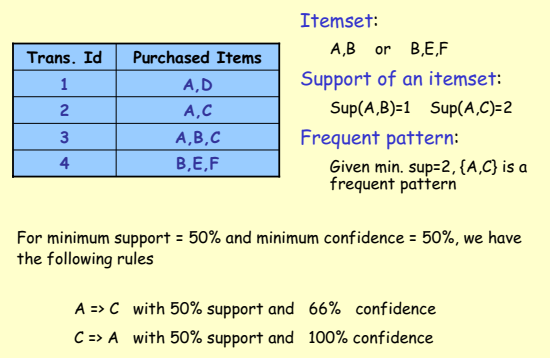
\includegraphics[scale=0.75]{images/lec08-pic04.png}
	\end{figure}
\end{frame}

\begin{frame}{Математические обозначения}
	$X$ -- пространство объектов;

	$F = {f_1, \ldots, f_n}, f_i: X \rightarrow {0, 1}$ -- бинарные признаки (items);

	$X^l=\{x_1, \ldots, x_l\} \subset X$ -- обучающая выборка.

	Каждому подмножеству $\varphi \subseteq F$ соответствует конъюнкция

	\[\varphi(x)=\bigwedge \limits_{f\in \varphi} f(x), x \in X\]

	Если $\varphi(x)=1$, то <<признаки из $\varphi$ совместно встречаются в $x$>>/

	Поддержка (support) $\varphi$ в выборке $X^l$

	\[\nu(\varphi)=\frac{1}{l}\sum_{i=1}^{l}\varphi(x_i)\]

	Если $\nu(\varphi)\geq \delta$, то <<набор $\varphi$ частый>> (frequent itemset).

	Параметр $\delta$ -- минимальная поддержка, (min support).
\end{frame}

\begin{frame}{Математические обозначения}
	\begin{block}{Определение}
		Ассоциативное правило (association rule) $\varphi \rightarrow y$ -- это пара непересекающихся наборов $\varphi, y \subseteq F$, таких, что:
		\begin{enumerate}
			\item наборы $\varphi$ и $y$ совместно часто встречаются,
			\[\nu(\varphi \cup y) \geq \delta; \]
			\item если встречаются $\varphi$, то часто встречается также и $y$:
			\[\nu(y | \varphi) \equiv \frac{\nu(\varphi \cup y)}{\nu(\varphi)} \geq \chi\]		
		\end{enumerate}
	\end{block}
	
	$\nu(y | \varphi)$ -- значимость (confidence) правила.
	
	Параметр $\delta$ -- минимальная поддержка (min support).

	Параметр $\chi$ -- минимальная значимость (min conf).
\end{frame}

\section{Алгоритм Apriori}

\begin{frame}
  \frametitle{Содержание лекции}
  \tableofcontents[current]
\end{frame}

\begin{frame}{Логические (булевые) ассоциативные правила}
	\begin{figure}[h]
		\centering
		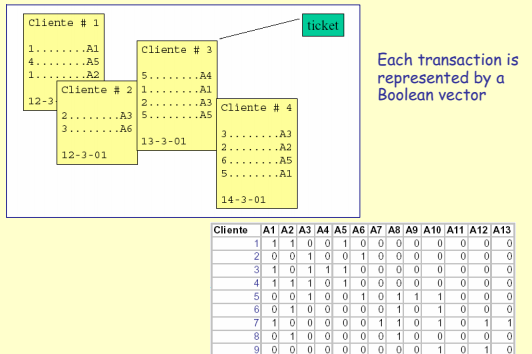
\includegraphics[scale=0.75]{images/lec08-pic07.png}
	\end{figure}
\end{frame}

\begin{frame}{Пример поиска ассоциативных правил}
	\begin{figure}[h]
		\centering
		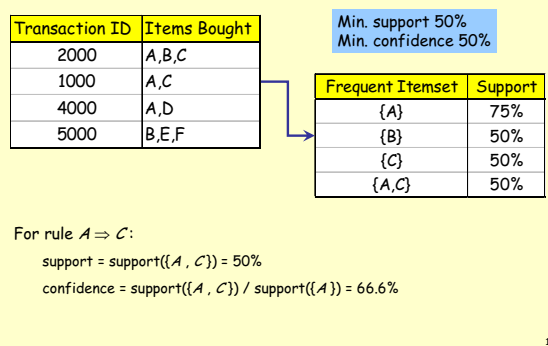
\includegraphics[scale=0.75]{images/lec08-pic08.png}
	\end{figure}
\end{frame}

\begin{frame}{Принцип Apriori}
	\begin{figure}[h]
		\centering
		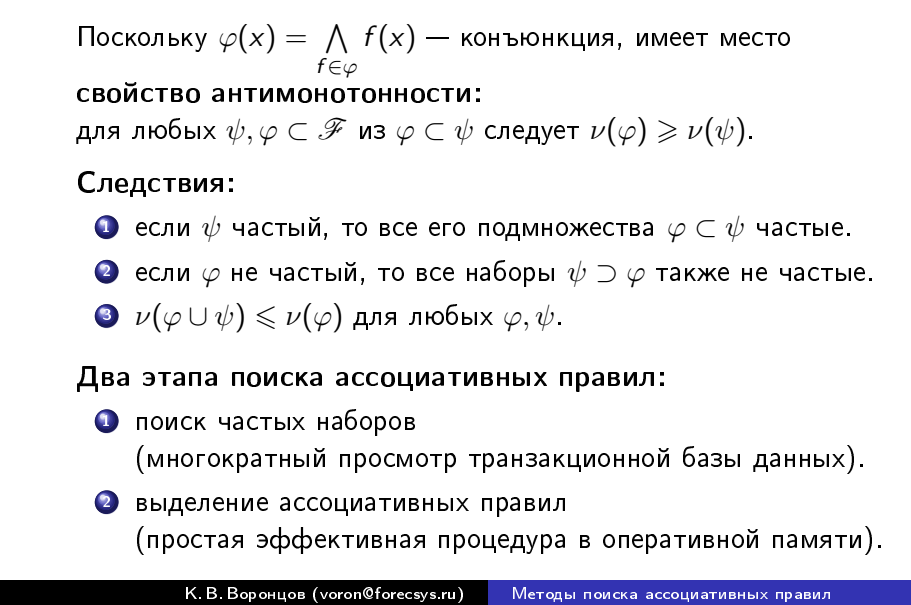
\includegraphics[scale=0.45]{images/lec08-pic09.png}
	\end{figure}
\end{frame}

\begin{frame}{Принцип Apriori: множество наборов}
	\begin{figure}[h]
		\centering
		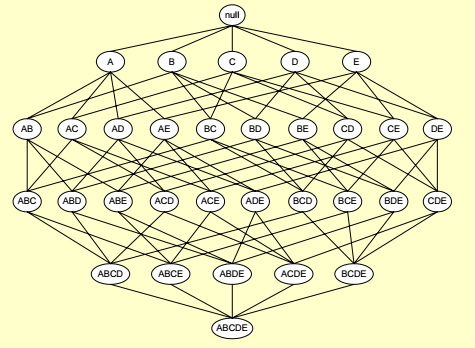
\includegraphics[scale=0.75]{images/lec08-pic10.png}
	\end{figure}
\end{frame}

\begin{frame}{Принцип Apriori: не рассматриваемые наборы}
	\begin{figure}[h]
		\centering
		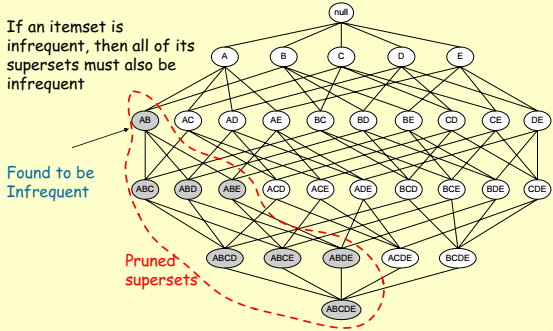
\includegraphics[scale=0.75]{images/lec08-pic11.png}
	\end{figure}
\end{frame}

\begin{frame}{Принцип Apriori: основная идея -- поиск в ширину}
	\begin{figure}[h]
		\centering
		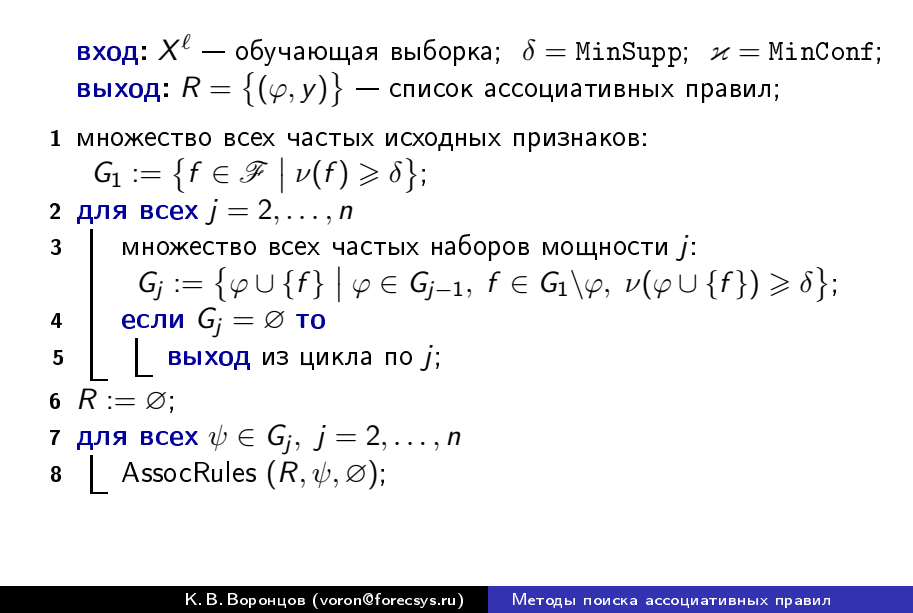
\includegraphics[scale=0.5]{images/lec08-pic12.png}
	\end{figure}
\end{frame}

\begin{frame}{Принцип Apriori: пример}
	\begin{figure}[h]
		\centering
		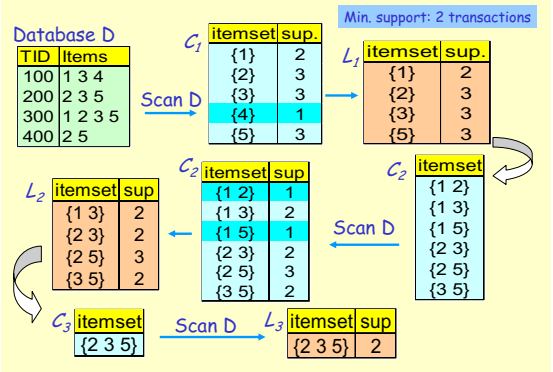
\includegraphics[scale=0.75]{images/lec08-pic13.png}
	\end{figure}
\end{frame}

\begin{frame}{Принцип Apriori: пример}
	\begin{figure}[h]
		\centering
		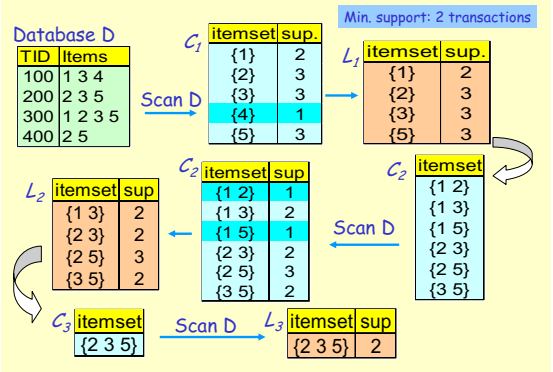
\includegraphics[scale=0.75]{images/lec08-pic13.png}
	\end{figure}
\end{frame}

\begin{frame}{Принцип Apriori: получение ассоциативных правил}
	\begin{figure}[h]
		\centering
		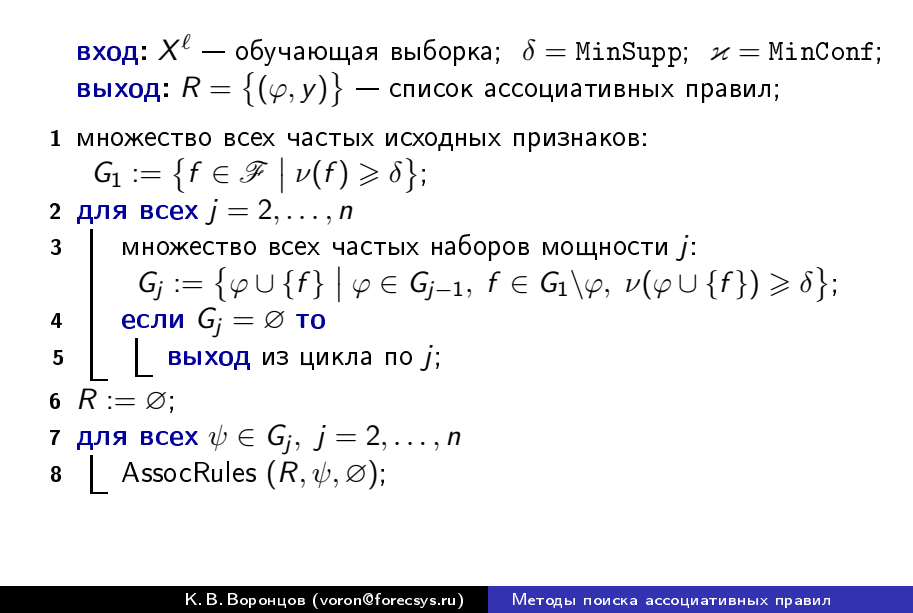
\includegraphics[scale=0.5]{images/lec08-pic12.png}
	\end{figure}
\end{frame}

\begin{frame}{Выделение ассоциативных правил}
	\[confidence(A\Rightarrow B)= P(B|A) = support(A\cup B)/support(A)\]

	\begin{itemize}
		\item Для каждого частого набора элементов $x$ сгенерировать все непустые подмножества $x$;
		\item Для каждого непустого подмножества $x$ множества s получить правило:
	\end{itemize}
	
	\[s \Rightarrow (s\setminus x)\]
	если
	\[support(x)/support(s) > MinConf\]
\end{frame}

\begin{frame}{Выделение ассоциативных правил}
%	\begin{figure}
%		\centering
		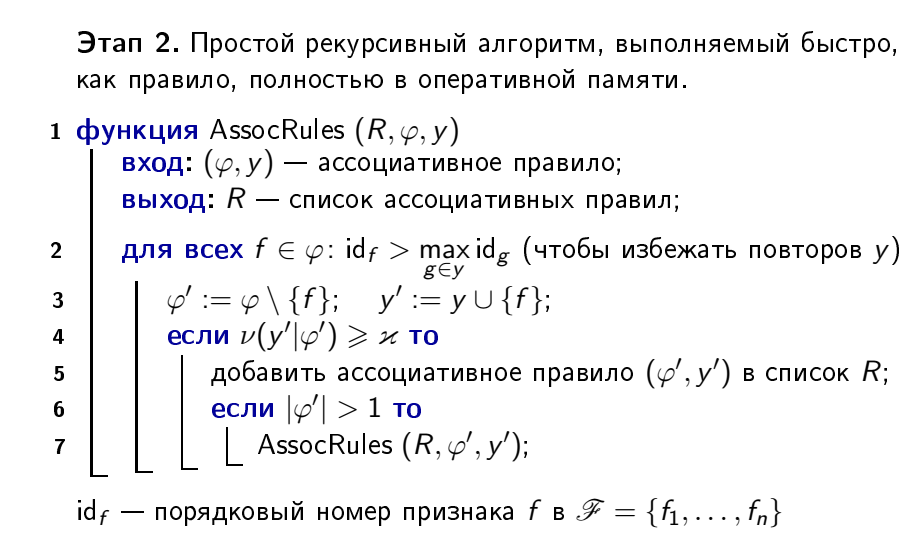
\includegraphics[scale=0.5]{images/lec08-pic14.png}
%	\end{figure}
\end{frame}

\begin{frame}{Пример}
	Задан часто встречающийся набор (A, B, E). Какие возможны ассоциативные правила?
	\begin{figure}[h]
		\centering
		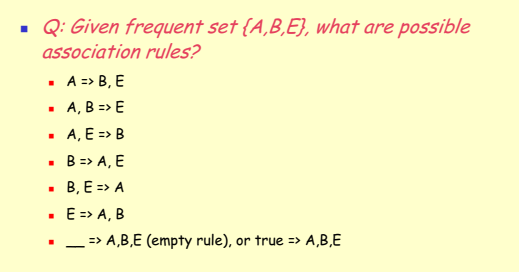
\includegraphics[scale=0.75]{images/lec08-pic15.png}
	\end{figure}
\end{frame}

\begin{frame}{Пример}
	\begin{figure}[h]
		\centering
		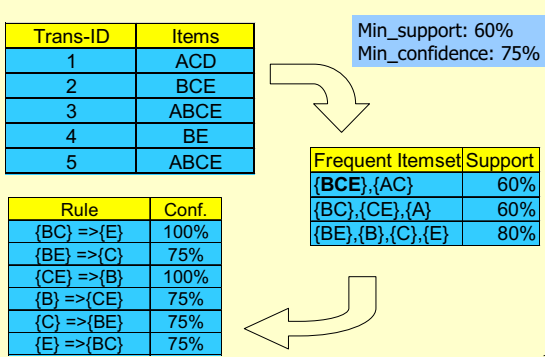
\includegraphics[scale=0.75]{images/lec08-pic16.png}
	\end{figure}
\end{frame}

\begin{frame}{Упражнение}
	\begin{figure}[h]
		\centering
		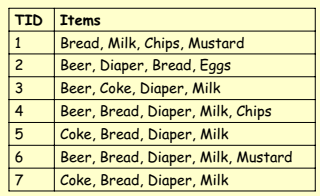
\includegraphics[scale=1]{images/lec08-pic17.png}
	\end{figure}
\end{frame}

\begin{frame}{Упражнение}
	\begin{figure}[h]
		\centering
		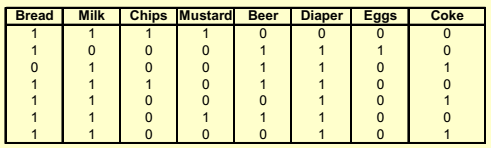
\includegraphics[scale=0.8]{images/lec08-pic18.png}
	\end{figure}
\end{frame}

\begin{frame}{Упражнение}
	\begin{figure}[h]
		\centering
		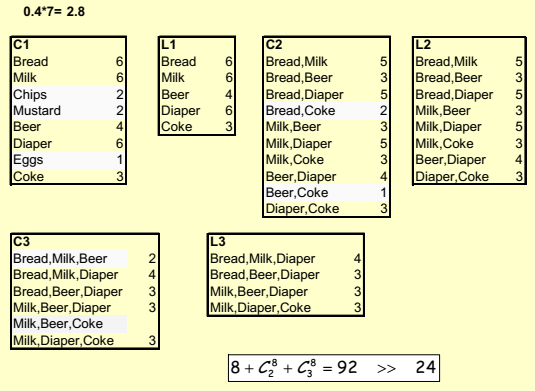
\includegraphics[scale=0.75]{images/lec08-pic19.png}
	\end{figure}
\end{frame}

\begin{frame}{Модификация алгоритма Apriori}
	Основные проблемы при генерации наборов:
	\begin{itemize}
		\item общее число транзакций может быть \textbf{очень большим};
		\item одна транзакция может содержать \textbf{много элементов}.
	\end{itemize}
	
	Модификации алгоритма:
	\begin{itemize}
		\item более эффективные структуры данных для быстрого поиска;
		\item поиск по частичной случайной выборке при пониженных поддержке и значимости с последующей проверкой на полной базе;
		\item алгоритмы, учитывающие иерархию признаков;
		\item поиск последовательных шаблонов;
	\item учет информации о клиентах.
	\end{itemize}
\end{frame}

\begin{frame}{Модификации алгоритма Apriori}
	\begin{itemize}
		\item \textbf{Проблема}: на каждом уровне осуществляется просмотр всей базы данных транзакций
		\item \textbf{AprioriTID}: 
  		\begin{itemize}
  			\item генерировать набора как в алгоритме Аpriori, но БД используется для вычисления поддержки всех наборов за один проход;
  			\item требуется значительно больше памяти;
  			\item вычисляются и хранятся часто встречающиеся наборы $C\hat{\text{ }}_k$ для каждой транзакции;
		\end{itemize}
		\item \textbf{AprioriHybrid} 
  		\begin{itemize}
  			\item на начальном этапе используется алгоритм Apriori;
			\item вычисляется размер $C\hat{\text{ }}_k$; 
  			\item как только $C\hat{\text{ }}_k$ будет умещаться в памяти, переключиться на AprioriTid.
  		\end{itemize}
	\end{itemize}
\end{frame}

\begin{frame}[t]{Какие правила интересны?}
	\begin{itemize}
		\item все ли найденные правила будут полезны и интересны?
		\item как можно измерить <<интересность>> правила?
	\end{itemize}

	Субъективные критерии:
	\begin{enumerate}
		\item правило интересно, если оно неожиданно для пользователя;
		\item правило полезно, если пользователь может его применить.
	\end{enumerate}

	Объективные критерии:
	\begin{enumerate}
		\item поддержка (Support)
		\item значимость (Confidence)
		\item интересность (Lift, Interest, Correlation) 
		\item убедительность (Conviction)
		\item влияние (Leverage, Piatetsky-Shapiro)
		\item покрытие (Coverage)	
	\end{enumerate}
\end{frame}

\begin{frame}{Пример}
	Среди 5000 студентов:
	\begin{itemize}
		\item 3000 играют в баскетбол;
		\item 3750 едят хлопья;
		\item 2000 и играют в баскетбол, и едят хлопья.					
	\end{itemize}

	\center{play basketball $\rightarrow$ eat cereal [40\%, 66.7\%]}	
	

	\center{play basketball $\rightarrow$ not eat cereal [20\%, 33.3\%]}
	
	\begin{figure}[h]
		\centering
		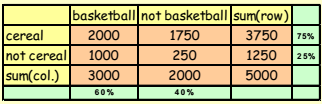
\includegraphics[scale=1]{images/lec08-pic21.png}
	\end{figure}
\end{frame}

\begin{frame}{Пример}
	Lift (Correlation, Interest):
	\[Lift(A \rightarrow B)=\frac{sup(A,B)}{sup(A)\cdot sup(B)}=\frac{P(B|A)}{P(B)}\]
	
	A и B имеют отрицательную корреляцию, если значение $Lift<1$, иначе корреляция положительная.

	\begin{figure}[h]
		\centering
		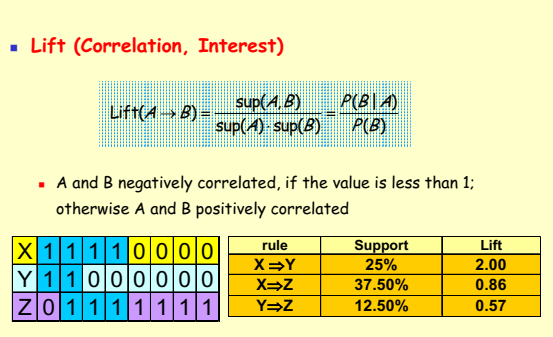
\includegraphics[scale=0.8]{images/lec08-pic22.png}
	\end{figure}
\end{frame}

\begin{frame}{Пример}
	Продолжение примера:
	\begin{itemize}
		\item play basketball => eat cereal [40\%, 66.7\%]
		\[ Lift=\frac{\frac{2000}{5000}}{\frac{3000}{5000} \times \frac{3750}{5000}} = 0.89\]
		\item play basketball => not eat cereal [20\%, 33.3\%]
		\[ Lift=\frac{\frac{1000}{5000}}{\frac{3000}{5000} \times \frac{1250}{5000}} = 1.33\]
	\end{itemize}	
	\begin{figure}[h]
		\centering
		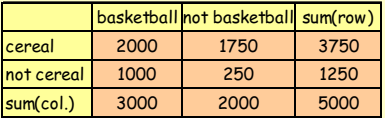
\includegraphics[scale=0.7]{images/lec08-pic23.png}
	\end{figure}
\end{frame}

\begin{frame}{Убедительность}
	\textbf{Убедительность} -- мера импликации, ее значение равно 1, если элементы не связаны.
	\[
	Conv(A\rightarrow B)=\frac{sup(A\cdot sup(\neg B)}{sup(A,\neg B)}=\frac{P(A)\cdot P(\neg B)}{P(A, \neg B)}=\frac{P(A)(1-P(B))}{P(A)-P(A,B)}
	\]
	Замечание: $A \rightarrow B$ можно записать в виде $\neg(A,\neg B)$.	
	\begin{itemize}
		\item play basketball => eat cereal [40\%, 66.7\%]
		\item eat cereal => play basketball conv: 0.85		
		\[Conv=\frac{\frac{3000}{5000}\left(1-\frac{3750}{5000}\right)}{\frac{3000}{5000}-\frac{2000}{5000}} = 0.75\]
		\item play basketball => not eat cereal [20\%, 33.3\%]
		\item not eat cereal => play basketball conv: 1.43
		\[Conv=\frac{\frac{3000}{5000}\left(1-\frac{1250}{5000}\right)}{\frac{3000}{5000}-\frac{1000}{5000}} = 1.125\]
	\end{itemize}
\end{frame}

\begin{frame}{Влияние}
	\begin{block}{Влияние (Leverage, Piatetsky-Shapiro, PS)}
		мера зависимости предпосылки и следствия.
		
		\[PS(A \rightarrow B)=sup(A,B)-sup(A)\cdot sup(B)\]		
	\end{block}

	\begin{block}{Покрытие (coverage)}			
		\[Coverage(A \rightarrow B)=sup(A)\]		
	\end{block}	
\end{frame}

\section{Алгоритм FP-Growth}

\begin{frame}
  \frametitle{Содержание лекции}
  \tableofcontents[current]
\end{frame}

\begin{frame}{Префиксное FP-дерево (FP-frequent pattern)}
	\begin{figure}[h]
		\centering
		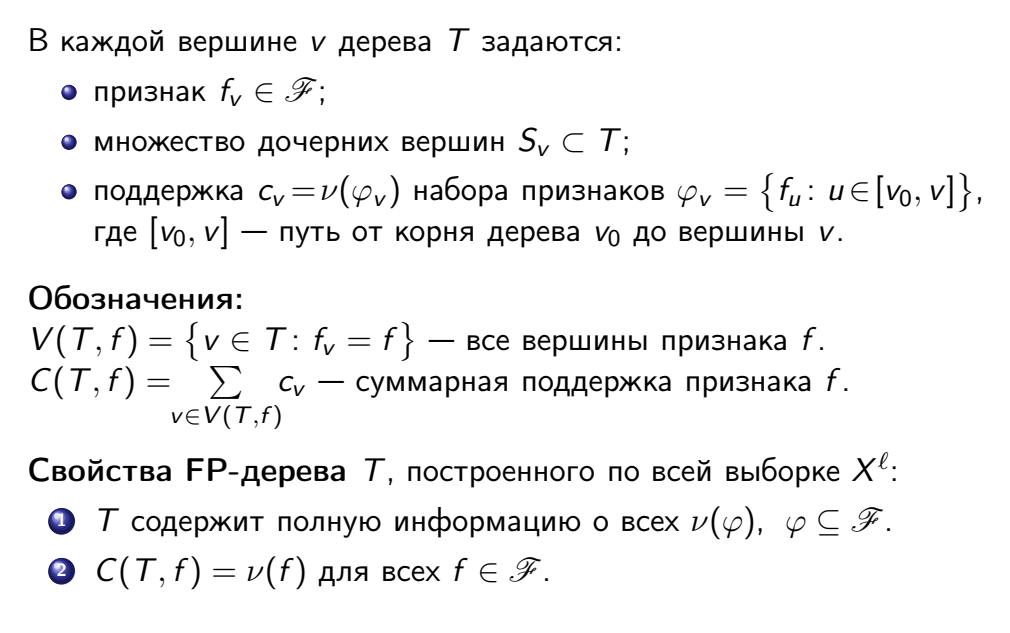
\includegraphics[scale=0.45]{images/lec08-pic31.png}
	\end{figure}
\end{frame}

\subsection{Пример: построение FP-дерева}

\begin{frame}
	\begin{figure}[h]
		\centering
		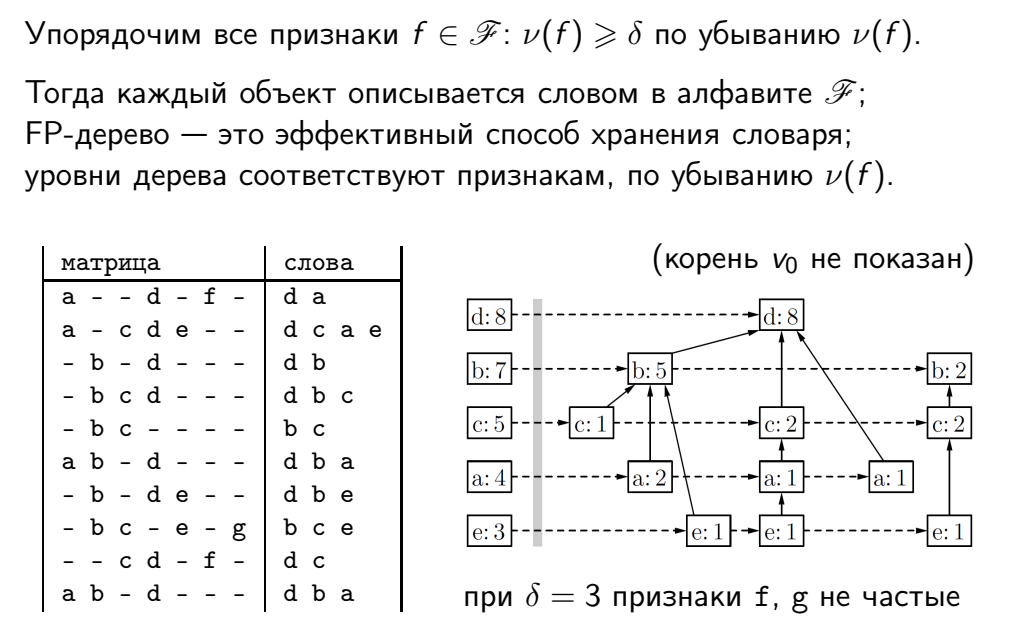
\includegraphics[scale=0.45]{images/lec08-pic32.png}
	\end{figure}
\end{frame}

\begin{frame}
	\begin{figure}[h]
		\centering
		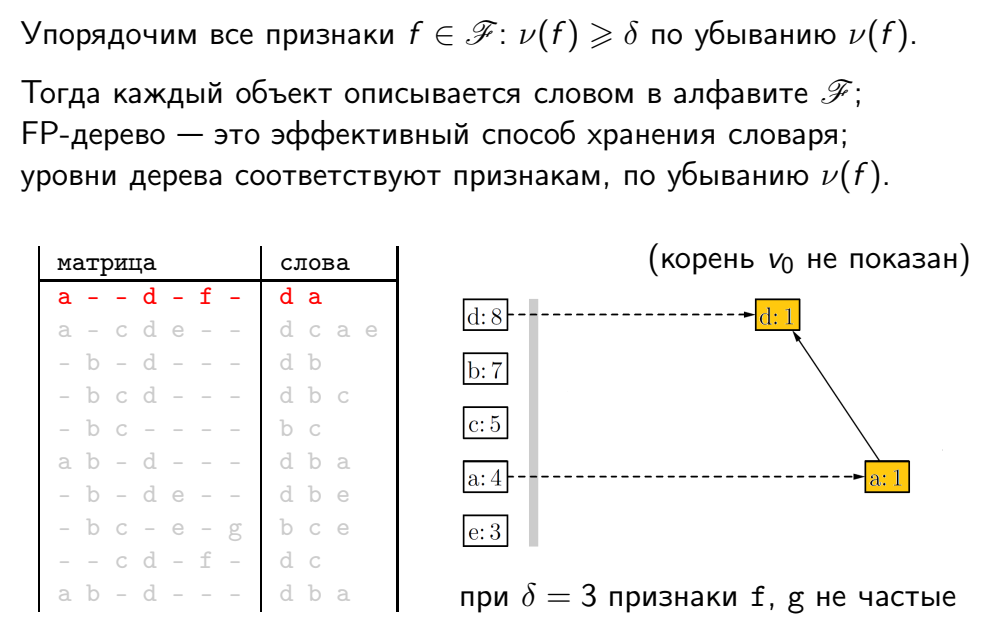
\includegraphics[scale=0.45]{images/lec08-pic33.png}
	\end{figure}
\end{frame}

\begin{frame}
	\begin{figure}[h]
		\centering
		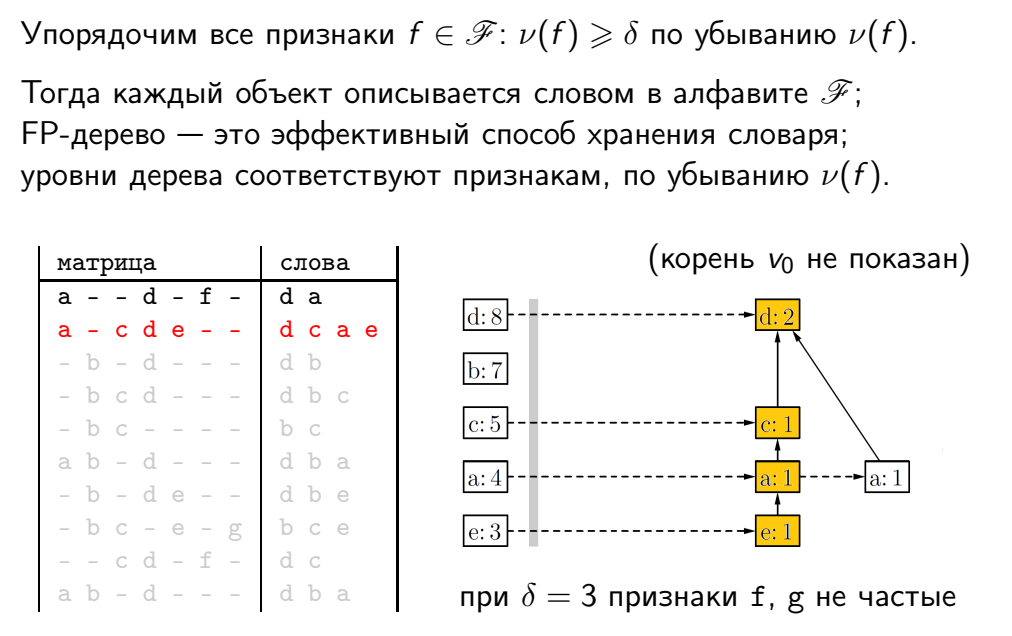
\includegraphics[scale=0.45]{images/lec08-pic34.png}
	\end{figure}
\end{frame}

\begin{frame}
	\begin{figure}[h]
		\centering
		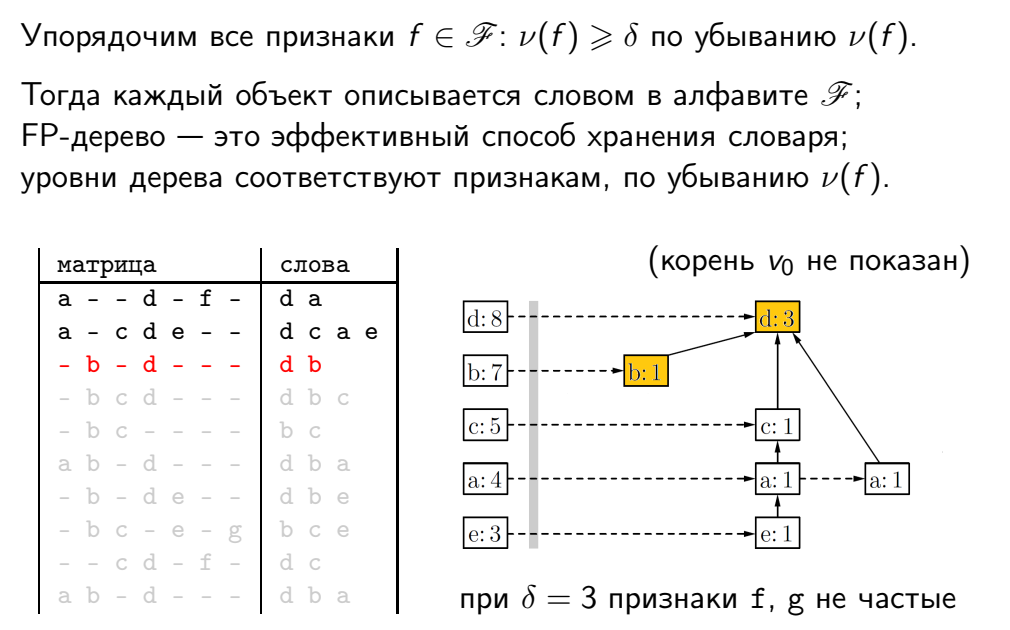
\includegraphics[scale=0.45]{images/lec08-pic35.png}
	\end{figure}
\end{frame}

\begin{frame}
	\begin{figure}[h]
		\centering
		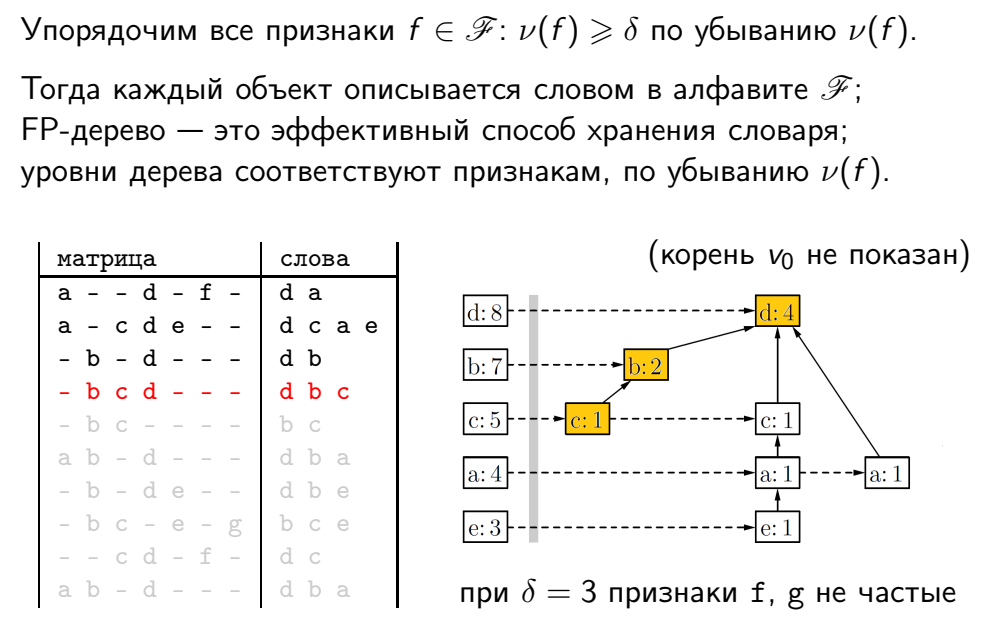
\includegraphics[scale=0.45]{images/lec08-pic36.png}
	\end{figure}
\end{frame}

\begin{frame}
	\begin{figure}[h]
		\centering
		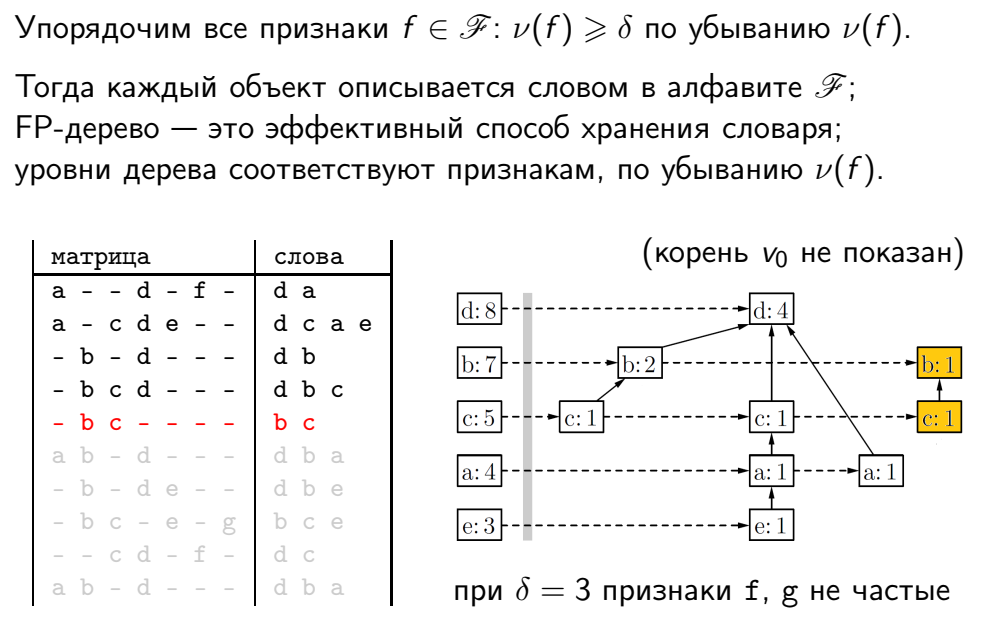
\includegraphics[scale=0.45]{images/lec08-pic37.png}
	\end{figure}
\end{frame}

\begin{frame}
	\begin{figure}[h]
		\centering
		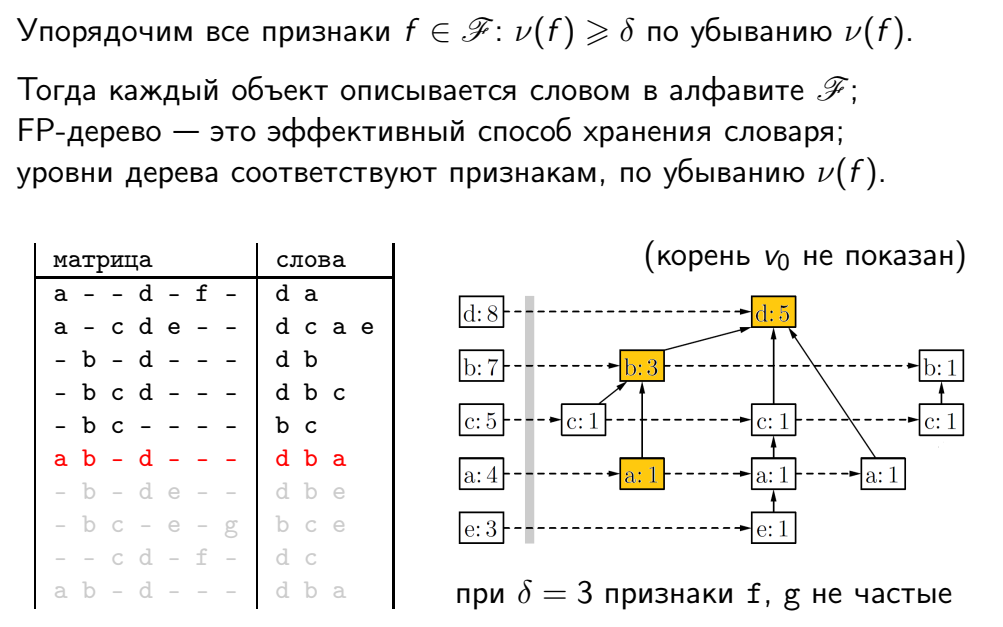
\includegraphics[scale=0.45]{images/lec08-pic38.png}
	\end{figure}
\end{frame}

\begin{frame}
	\begin{figure}[h]
		\centering
		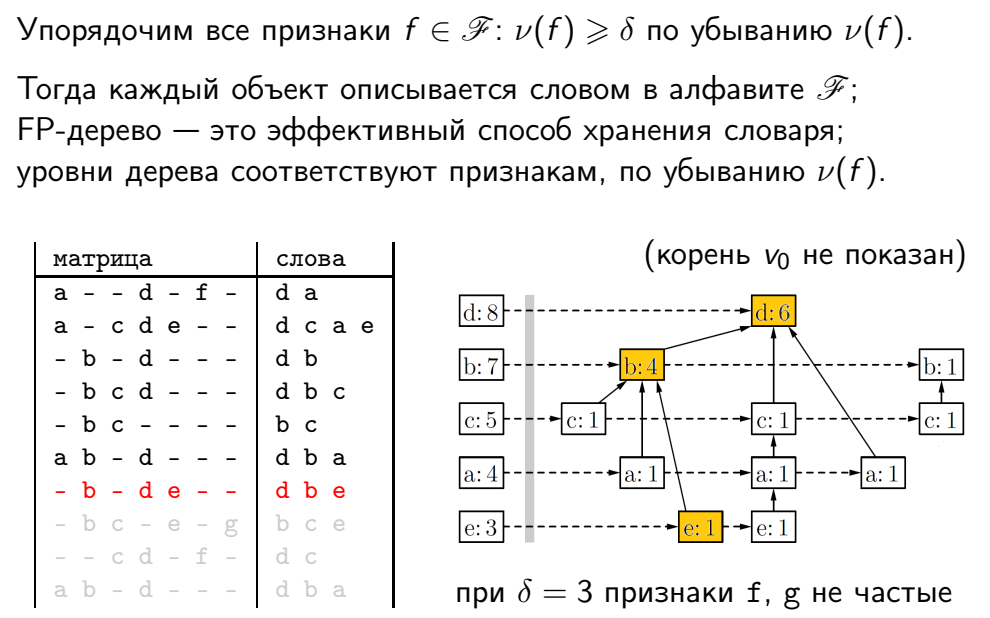
\includegraphics[scale=0.45]{images/lec08-pic39.png}
	\end{figure}
\end{frame}

\begin{frame}
	\begin{figure}[h]
		\centering
		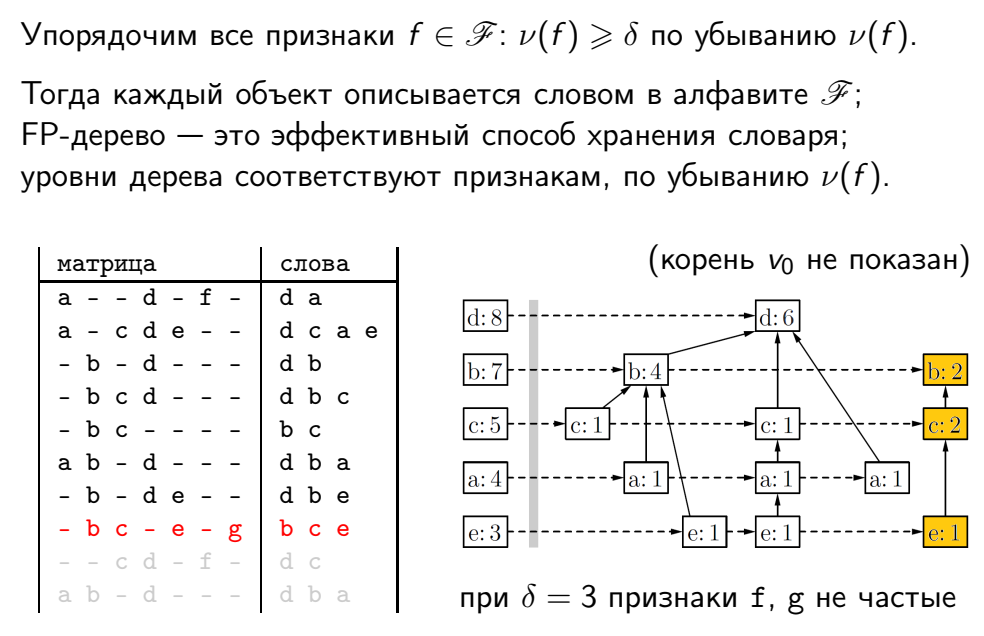
\includegraphics[scale=0.45]{images/lec08-pic40.png}
	\end{figure}
\end{frame}

\begin{frame}
	\begin{figure}[h]
		\centering
		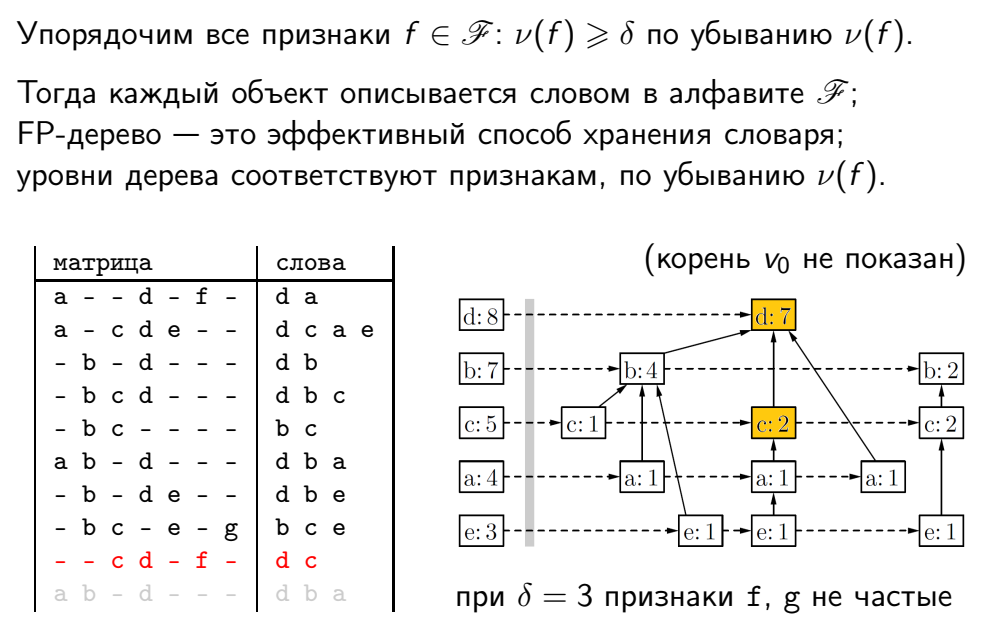
\includegraphics[scale=0.45]{images/lec08-pic41.png}
	\end{figure}
\end{frame}

\begin{frame}
	\begin{figure}[h]
		\centering
		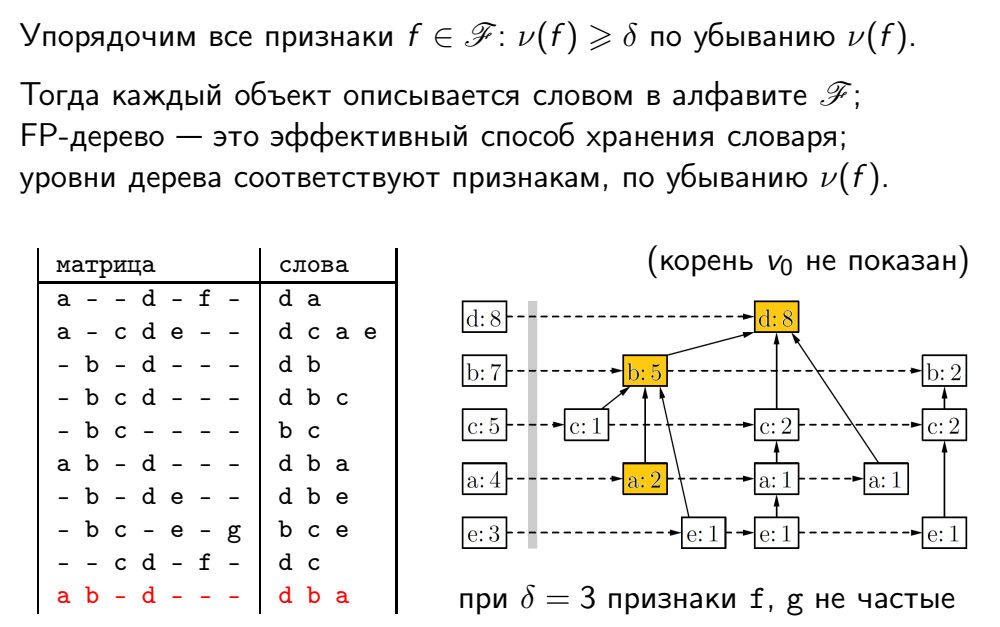
\includegraphics[scale=0.45]{images/lec08-pic42.png}
	\end{figure}
\end{frame}

\subsection{Алгоритм построения FP-дерева}

\begin{frame}
	\begin{figure}[h]
		\centering
		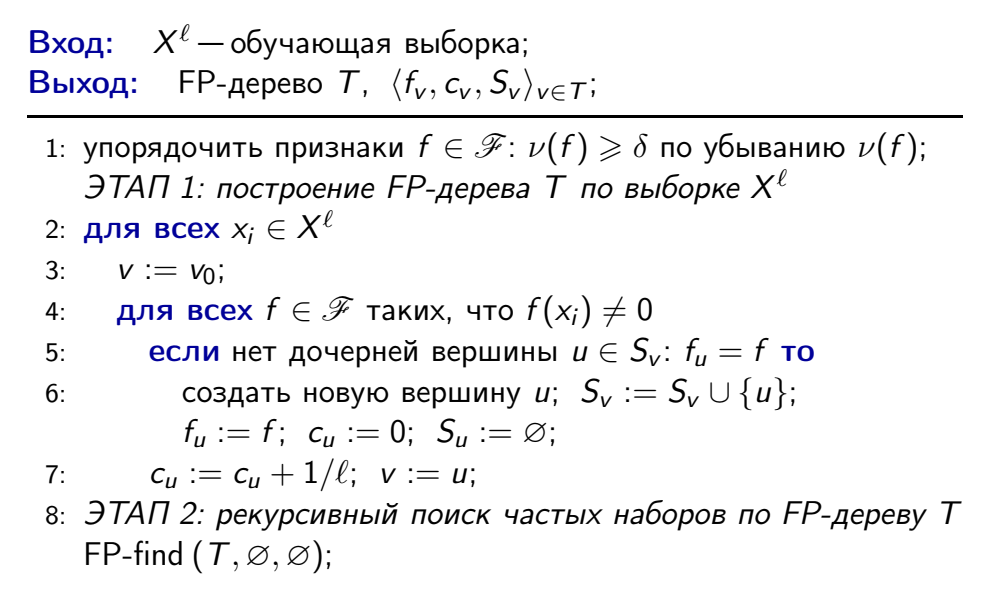
\includegraphics[scale=0.45]{images/lec08-pic43.png}
	\end{figure}
\end{frame}

\subsection{Рекурсивный поиск часто встречащихся наборов по FP-дереву}

\begin{frame}
	\begin{figure}[h]
		\centering
		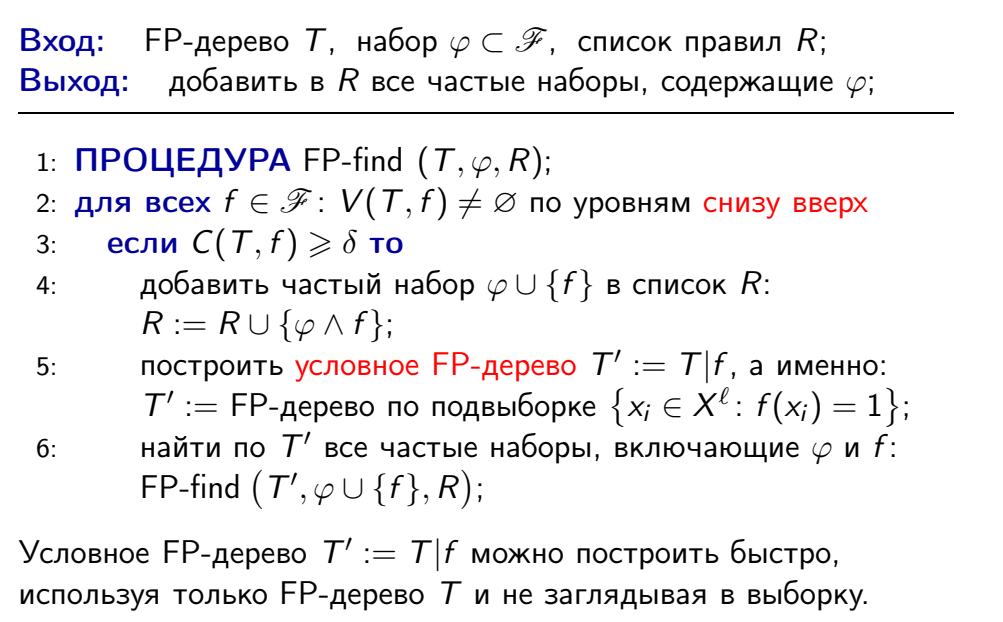
\includegraphics[scale=0.45]{images/lec08-pic44.png}
	\end{figure}
\end{frame}

\subsection{Условное FP-дерево}

\begin{frame}
	\begin{figure}[h]
		\centering
		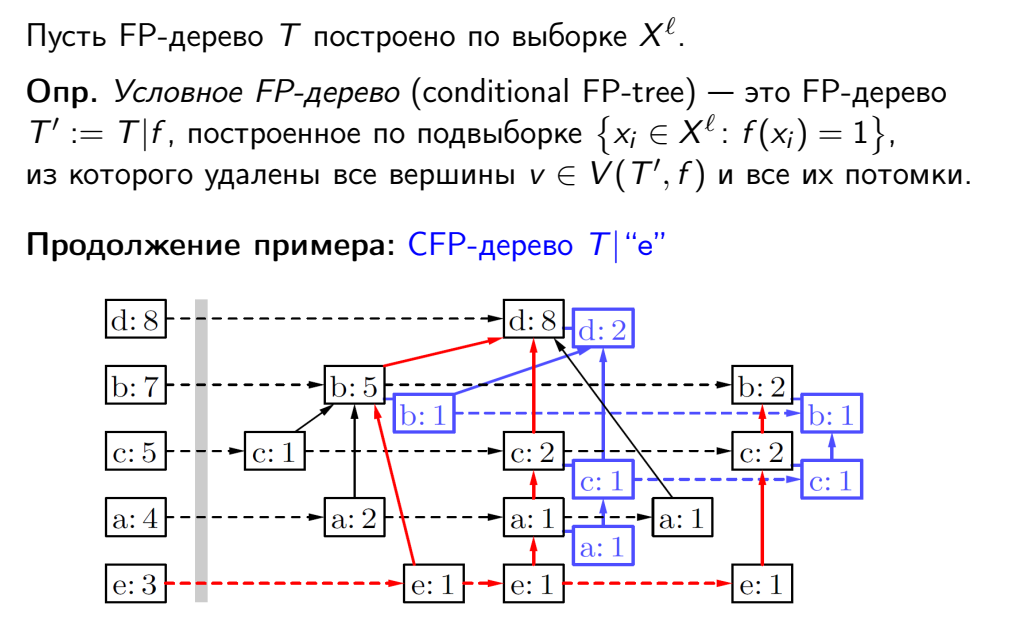
\includegraphics[scale=0.45]{images/lec08-pic45.png}
	\end{figure}
\end{frame}

\subsection{Быстрое построение условного FP-дерева}

\begin{frame}
	\begin{figure}[h]
		\centering
		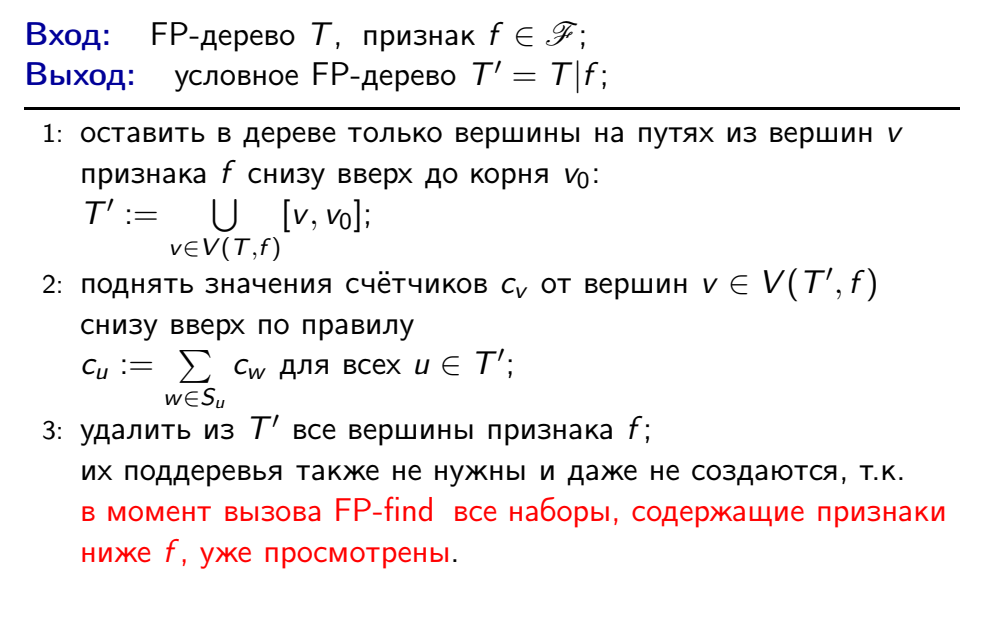
\includegraphics[scale=0.45]{images/lec08-pic46.png}
	\end{figure}
\end{frame}

\subsection{Эффективность алгоритма FP-Growth}

\begin{frame}
	\begin{figure}[h]
		\centering
		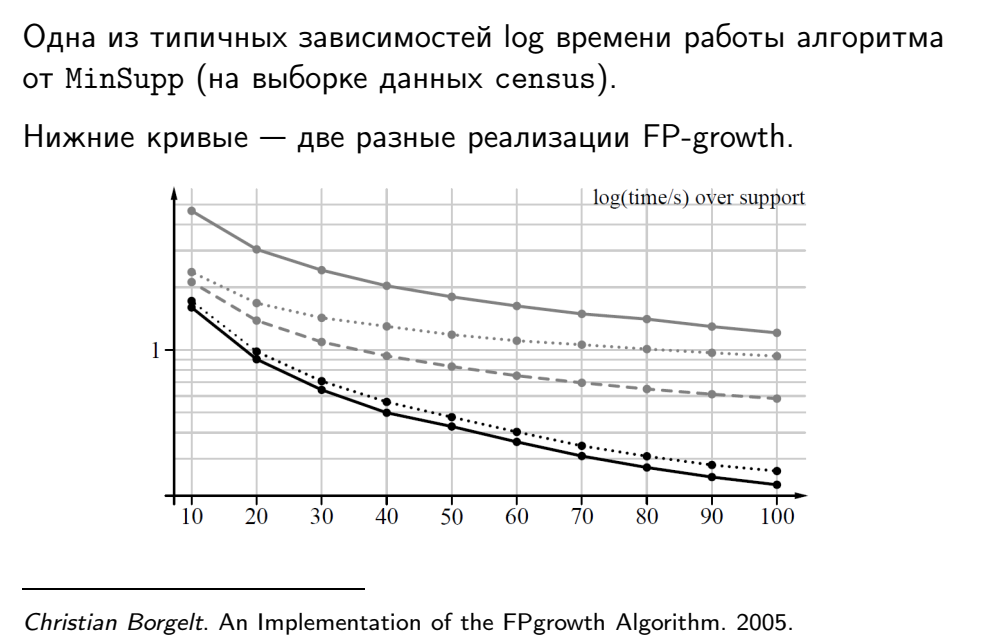
\includegraphics[scale=0.45]{images/lec08-pic47.png}
	\end{figure}
\end{frame}

\section{Визуализация ассоциативных правил}

\begin{frame}
  \frametitle{Содержание лекции}
  \tableofcontents[current]
\end{frame}

\begin{frame}{Визуализация ассоциативных правил}
	\begin{figure}[h]
		\centering
		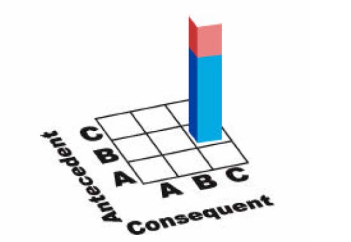
\includegraphics[scale=0.7]{images/lec08-pic27.png}
	\end{figure}
\end{frame}

\begin{frame}{Визуализация ассоциативных правил}
	\begin{figure}[h]
		\centering
		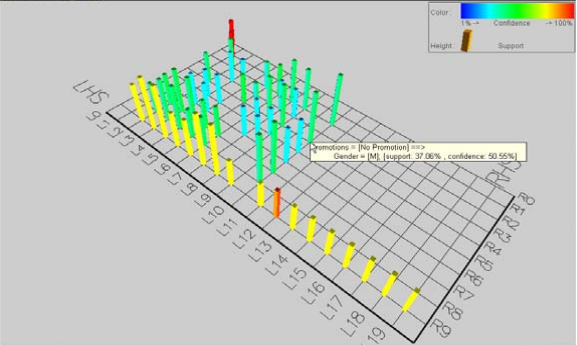
\includegraphics[scale=0.7]{images/lec08-pic28.png}
	\end{figure}
\end{frame}

\begin{frame}{Визуализация ассоциативных правил}
	\begin{figure}[h]
		\centering
		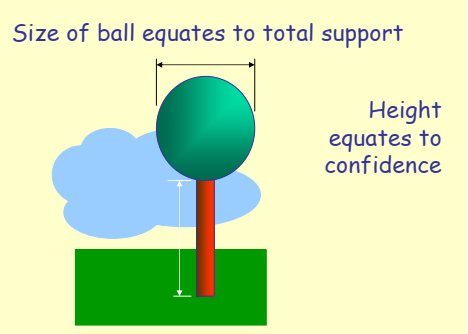
\includegraphics[scale=0.75]{images/lec08-pic29.png}
	\end{figure}
\end{frame}

\begin{frame}{Визуализация ассоциативных правил}
	\begin{figure}[h]
		\centering
		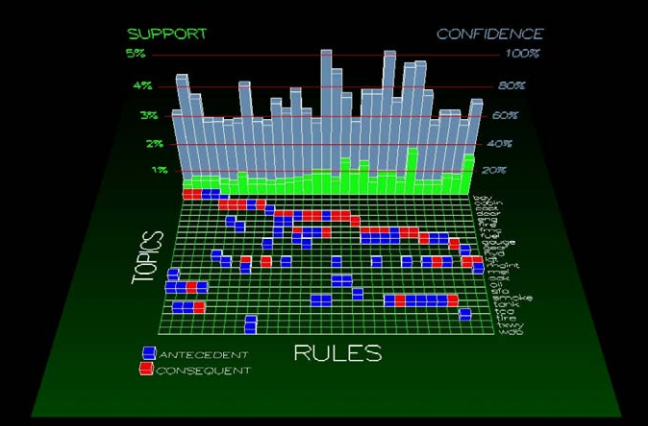
\includegraphics[scale=0.6]{images/lec08-pic30.png}
	\end{figure}
\end{frame}

\begin{frame}{Выводы}
	\begin{itemize}
		\item Поиск ассоциативных правил — обучение без учителя.
		\item Простые алгоритмы типа APriory вычислительно неэффективны на больших данных.
		\item FP-growth — один из самых эффективных алгоритмов поиска ассоциативных правил.
		\item Для практических приложений часто используются его инкрементные и/или иерархические обобщения.
	\end{itemize}
\end{frame}

\end{document}